\section{Cybersikkerhet}
\label{sec:cyber}


\subsection{PURDUE: Nettverksarkitektur}

PURDUE er en nettverksarkitektur med ulike nettverksnivåer, hvor hvert nivå har et eget nettverk. 

\begin{itemize}
    \item \textbf{Information Technology - del}:
    \begin{itemize}
        \item Nivå 4: Enterprise/kontornettverk
    \end{itemize}
    \item \textbf{Operational technology (styringssystemer) - del}:
    \begin{itemize}
        \item Nivå 3.5: DMZ (demillitarisert)-sone mellom nivå 4 og 3, eks brannmur. Fra wikipedia: En DMZ eller demilitarisert sone i datanettverk er et fysisk eller logisk subnet som offentliggjør en organisasjons offentlige tjenere mot internett. 
        \item Nivå 3: Servere til datainnsamling. 
        \item Nivå 2: Overvåkning (kontrollrom). Eget nettverk med kontrollert forbindelse.
        \item Nivå 1: Kontrollere (SIF-er og basic kontrollenheter)
        \item Nivå 0: Sensorer/prosessutstyr - busser, analoge signaler, IO-utstyr osv.
    \end{itemize}
\end{itemize}


\begin{figure}[H]
    \centering
        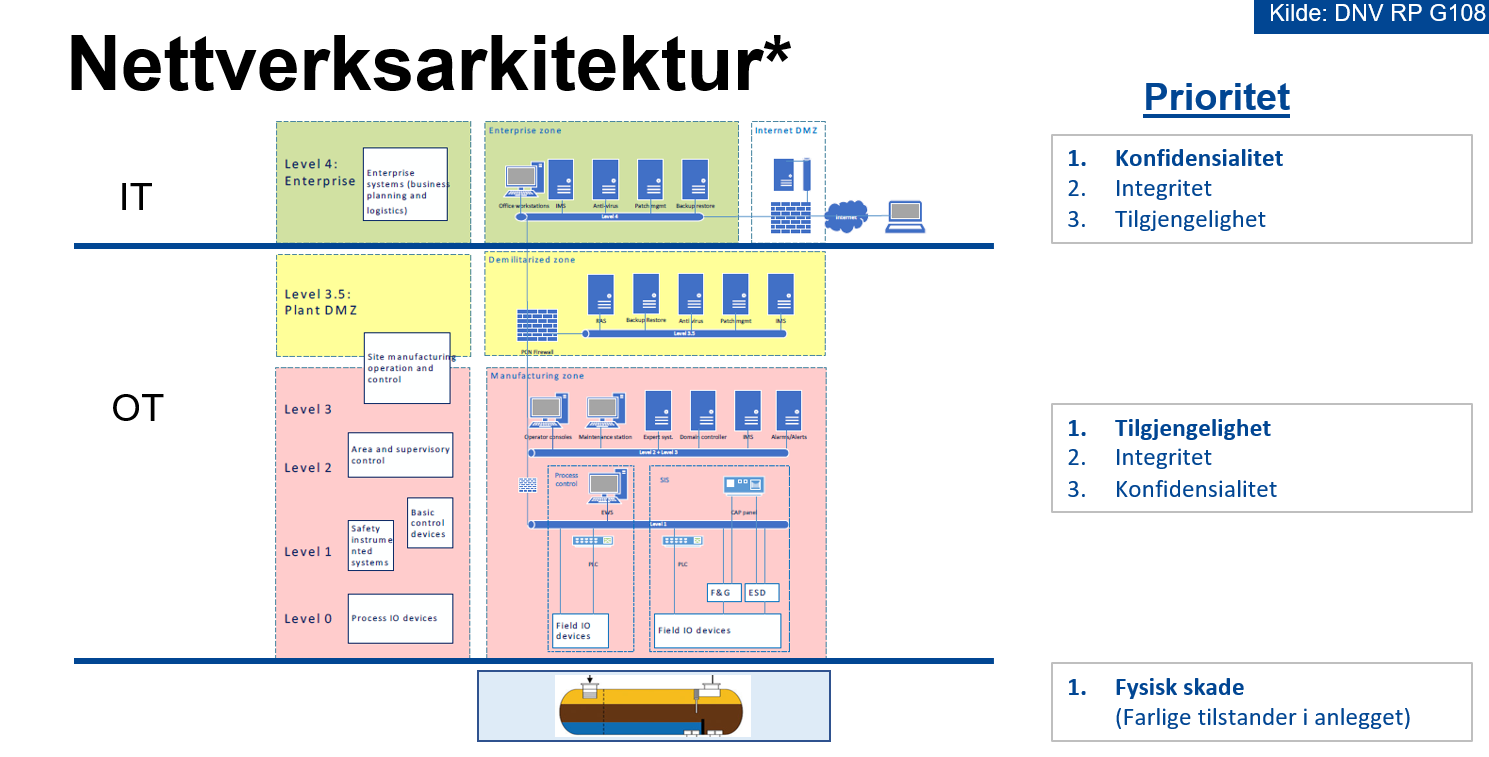
\includegraphics[width=\textwidth]{figures/cyber/purdue.PNG}\\
        \caption{PURDUE referansearkitektur.}
\end{figure}

\subsection{Beskyttelsestiltak}

IEC62443 er bibelen for standarder vedr. industrielle kommunikasjonsnettverk. I standarden defineres SL (security level) -krav, analogi til SIL-kravene, se figur. 

\begin{figure}[H]
    \centering
        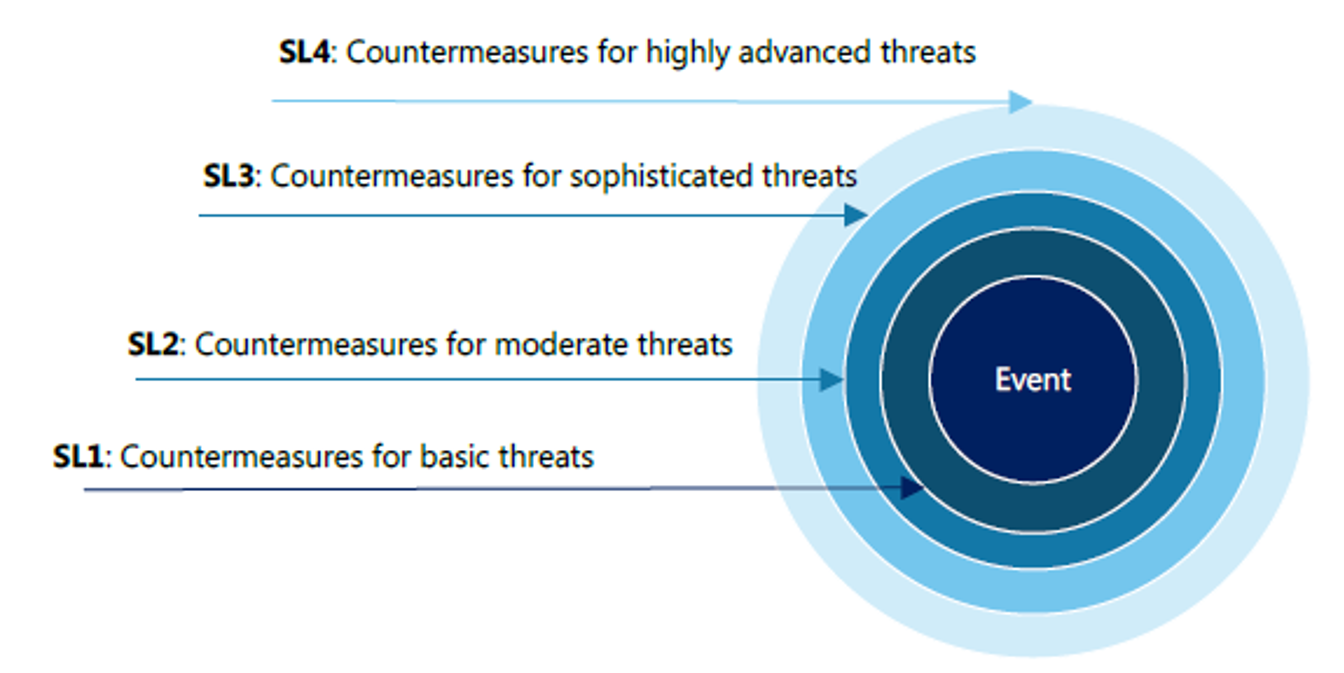
\includegraphics[width=\textwidth]{figures/cyber/sl-krave.PNG}\\
        \caption{De fire nivåene med SL-krav.}
\end{figure}

Standarden beskriver steg for å bestemme soneinndeling, tuneller mellom sonene, og SL-krav til sonene. Tommelfingerregler:

\begin{figure}[H]
    \centering
        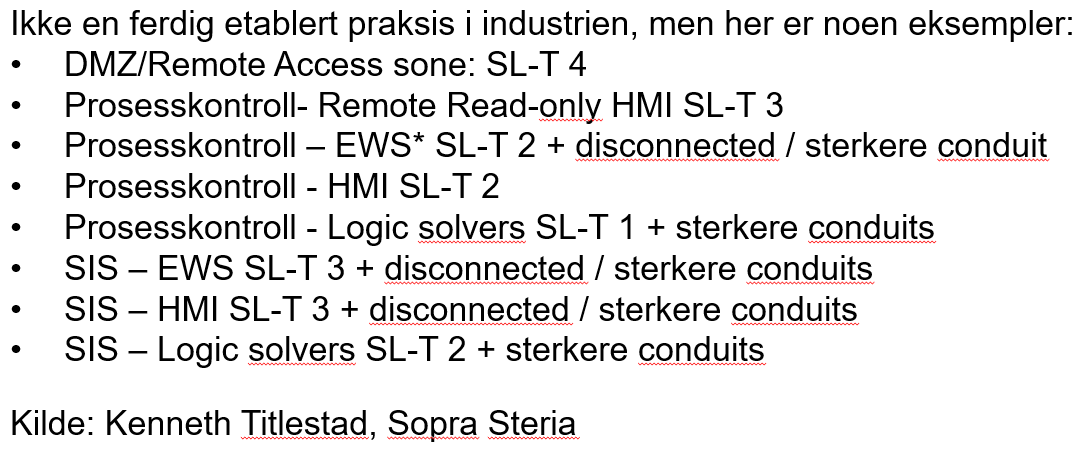
\includegraphics[width=\textwidth]{figures/cyber/tommel.PNG}\\
        \caption{Tommelfingerregler for SL-krav til soner.}
\end{figure}

IEC identiserer også ulike kategorier for beskyttelsestiltak:

\begin{itemize}
    \item [\textbf{FR 1}] – Identification and authentication control
    \item [\textbf{FR 2}] – Use control
    \item [\textbf{FR 3}] – System integrity 
    \item [\textbf{FR 4}] – Data confidentiality 
    \item [\textbf{FR 5}] – Restricted data flow
    \item [\textbf{FR 6}] – Timely response to events 
    \item [\textbf{FR 7}] – Resource availability
\end{itemize}


\subsection{CYPHASS-metoden}

CYPHASS-metoden er egentlig et komplekst bowtie-diagram som bidrar til å identifisere risiko for at feil forplanter seg fra cyberlaget og videre til det fysiske laget. På veien i analysen kan vi også identifisere deteksjon og sikkerhetsbarrierer for å hindre feilene i å forplante seg videre.